% Drawing 74/05-2 -- folder 74, batch 05, archive page 82 (PDF page 83).
% Transcription: Un triangle plein de sommet marqué, flanqué de deux segments pointillés.
% Kind: triangle with marked vertex and dotted segments. Method 2 (schematic redraw from the facsimile). Status: ok.
% Notes: A triangle in bold strokes, its lower vertex marked by a big dot, flanked by two dotted segments ending in points. The oval with « = » at the left belongs to the column of small marginal ovals (no mark of its own in the transcription).
% Coordinates: 1 unit = 1 mm = 1/100 of the crop width (bbox in page fractions: [0.1, 0.62, 0.25, 0.68]).
% Redrawn by Claude (claude-opus-5-5), issue #73, 2026-11-07; not checked by a human; not compiled (no TeX in the session).
% Rights: reproduces part of the work -- behind RENDER_TRANSCRIPTS, never published by itself.
\documentclass[tikz,border=3pt]{standalone}
\usepackage{amsmath,amssymb}
\usetikzlibrary{patterns,arrows.meta}
\tikzset{pencil/.style={black!45}, struck/.style={black!35}, mark/.style={circle,draw,inner sep=1.3pt}, pt/.style={circle,fill,inner sep=0.9pt}, opt/.style={circle,draw,fill=white,inner sep=1.1pt}}
\begin{document}
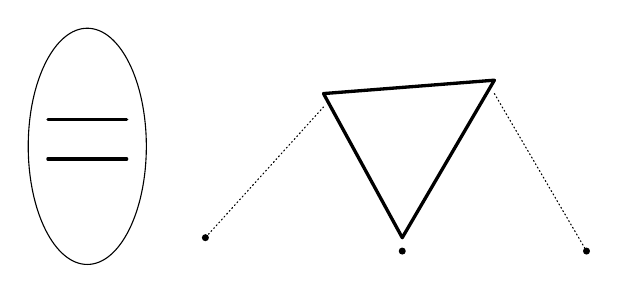
\begin{tikzpicture}[x=1mm,y=1mm,line cap=round,line join=round,font=\scriptsize]
\draw[very thick] (43.3,-21.9) -- (65,-20.2) -- (53.3,-40.2) -- cycle;
\node[pt] at (53.3,-41.9) {};
\draw[densely dotted] (43.3,-23.6) -- (28.3,-40.2);
\draw[densely dotted] (65,-21.9) -- (76.7,-41.9);
\node[pt] at (28.3,-40.2) {};
\node[pt] at (76.7,-41.9) {};
\draw (13.3,-28.6) ellipse[x radius=7.5, y radius=15];
\draw[very thick] (8.3,-25.2) -- (18.3,-25.2);
\draw[very thick] (8.3,-30.2) -- (18.3,-30.2);
\end{tikzpicture}
\end{document}
